\documentclass[hide notes,intlimits]{beamer}


\mode<presentation>
{
  \usetheme[headline,footline]{PISMshade}
  \setbeamercovered{transparent}
}

% load packages
\usepackage{multimedia}
\usepackage{animate}
\usepackage[english]{babel}
\usepackage[latin1]{inputenc}
\usepackage[T1]{fontenc}
\usepackage{lmodern}
\usepackage[multidot]{grffile}
\usepackage[amssymb]{SIunits}
% \usepackage{flashmovie}
\usepackage{tikz}
\usetikzlibrary{shapes,arrows,shadows, calc}

% \usepackage{pgfpages}
% \setbeamertemplate{note page}[plain]
% \setbeameroption{show notes on second screen=right}


\definecolor{dark red}{HTML}{E41A1C}
\definecolor{dark green}{HTML}{4DAF4A}
\definecolor{dark violet}{HTML}{984EA3}
\definecolor{dark blue}{HTML}{084594}
\definecolor{dark orange}{HTML}{FF7F00}
\definecolor{white}{HTML}{FFFFFF}
\definecolor{light blue}{HTML}{377EB8}
\definecolor{light red}{HTML}{FB9A99}
\definecolor{light violet}{HTML}{CAB2D6}

\definecolor{uaf red}{HTML}{E41A1C}
\definecolor{uaf blue}{HTML}{377EB8}
\definecolor{uaf green}{HTML}{4DAF4A}
\definecolor{uaf violet}{HTML}{984EA3}
\definecolor{uaf orange}{HTML}{FF7F00}
\setbeamercolor{boxed}{fg=black,bg=uaf yellow}


% Define block styles
\tikzstyle{initialization} = [ellipse, draw, 
    text badly centered, draw=dark violet,
        % The filling: 
        top color=white, 
        bottom color=dark violet]
\tikzstyle{initialization faded} = [ellipse, draw, 
    text badly centered, draw=dark violet!50,
        % The filling: 
        top color=white, 
        bottom color=dark violet!25]
\tikzstyle{hindcast} = [ellipse, draw,
    text badly centered, rounded corners,draw=dark orange,
        % The filling: 
        top color=white, 
        bottom color=dark orange]
\tikzstyle{hindcast faded} = [ellipse, draw,
    text badly centered, rounded corners,draw=dark orange!50,
        % The filling: 
        top color=white, 
        bottom color=dark orange!25]
\tikzstyle{forecast} = [ellipse, draw,
    text badly centered, rounded corners,draw=dark blue,
        % The filling: 
        top color=white, 
        bottom color=dark blue]
\tikzstyle{forecast faded} = [ellipse, draw,
    text badly centered, rounded corners,draw=dark blue!50,
        % The filling: 
        top color=white, 
        bottom color=dark blue!50]
\tikzstyle{arrow line} = [draw, -latex']
\tikzstyle{line} = [draw]



\graphicspath{{figures/}}

\setbeamerfont{caption}{size=\scriptsize}

% code adapted from http://tex.stackexchange.com/a/11483/3954

% some parameters for customization
\def\shadowshift{3pt,-3pt}
\def\shadowradius{6pt}

\colorlet{innercolor}{black!60}
\colorlet{outercolor}{gray!05}

% this draws a shadow under a rectangle node
\newcommand\drawshadow[1]{
    \begin{pgfonlayer}{shadow}
        \shade[outercolor,inner color=innercolor,outer color=outercolor] ($(#1.south west)+(\shadowshift)+(\shadowradius/2,\shadowradius/2)$) circle (\shadowradius);
        \shade[outercolor,inner color=innercolor,outer color=outercolor] ($(#1.north west)+(\shadowshift)+(\shadowradius/2,-\shadowradius/2)$) circle (\shadowradius);
        \shade[outercolor,inner color=innercolor,outer color=outercolor] ($(#1.south east)+(\shadowshift)+(-\shadowradius/2,\shadowradius/2)$) circle (\shadowradius);
        \shade[outercolor,inner color=innercolor,outer color=outercolor] ($(#1.north east)+(\shadowshift)+(-\shadowradius/2,-\shadowradius/2)$) circle (\shadowradius);
        \shade[top color=innercolor,bottom color=outercolor] ($(#1.south west)+(\shadowshift)+(\shadowradius/2,-\shadowradius/2)$) rectangle ($(#1.south east)+(\shadowshift)+(-\shadowradius/2,\shadowradius/2)$);
        \shade[left color=innercolor,right color=outercolor] ($(#1.south east)+(\shadowshift)+(-\shadowradius/2,\shadowradius/2)$) rectangle ($(#1.north east)+(\shadowshift)+(\shadowradius/2,-\shadowradius/2)$);
        \shade[bottom color=innercolor,top color=outercolor] ($(#1.north west)+(\shadowshift)+(\shadowradius/2,-\shadowradius/2)$) rectangle ($(#1.north east)+(\shadowshift)+(-\shadowradius/2,\shadowradius/2)$);
        \shade[outercolor,right color=innercolor,left color=outercolor] ($(#1.south west)+(\shadowshift)+(-\shadowradius/2,\shadowradius/2)$) rectangle ($(#1.north west)+(\shadowshift)+(\shadowradius/2,-\shadowradius/2)$);
        \filldraw ($(#1.south west)+(\shadowshift)+(\shadowradius/2,\shadowradius/2)$) rectangle ($(#1.north east)+(\shadowshift)-(\shadowradius/2,\shadowradius/2)$);
    \end{pgfonlayer}
}

% create a shadow layer, so that we don't need to worry about overdrawing other things
\pgfdeclarelayer{shadow} 
\pgfsetlayers{shadow,main}

\newsavebox\mybox
\newlength\mylen

\newcommand\shadowimage[2][]{%
\setbox0=\hbox{\includegraphics[#1]{#2}}
\setlength\mylen{\wd0}
\ifnum\mylen<\ht0
\setlength\mylen{\ht0}
\fi
\divide \mylen by 120
\def\shadowshift{\mylen,-\mylen}
\def\shadowradius{\the\dimexpr\mylen+\mylen+\mylen\relax}
\begin{tikzpicture}
\node[anchor=south west,inner sep=0] (image) at (0,0) {\includegraphics[#1]{#2}};
\drawshadow{image}
\end{tikzpicture}}

\newcommand\shadowimagec[3][]{%
\setbox0=\hbox{\includegraphics<#1>[#2]{#3}}
\setlength\mylen{\wd0}
\ifnum\mylen<\ht0
\setlength\mylen{\ht0}
\fi
\divide \mylen by 120
\def\shadowshift{\mylen,-\mylen}
\def\shadowradius{\the\dimexpr\mylen+\mylen+\mylen\relax}
\begin{tikzpicture}
\node[anchor=south west,inner sep=0] (image) at (0,0) {\includegraphics<#1>[#2]{#3}};
\drawshadow{image}
\end{tikzpicture}}


\newenvironment{transbox}[1][]{%
\begin{tikzpicture}
\node[drop shadow,rounded corners,text width=\textwidth,fill=white, fill opacity=#1,text opacity=1] \bgroup
}{
\egroup;\end{tikzpicture}} 

\newenvironment{transbox-tight}{%
\begin{tikzpicture}
\node[drop shadow,rounded corners,fill=uaf yellow, fill opacity=0.75,text opacity=1] \bgroup
}{
\egroup;\end{tikzpicture}} 


% title page
\title[] % (optional, use only with long paper titles)
{The Parallel Ice Sheet Model (PISM) and ISMIP6}



\author[Aschwanden] % (optional, use only with lots of authors)
{The PISM Team}
% - Give the names in the same order as the appear in the paper.
% - Use the \inst{?} command only if the authors have different
%   affiliation.

\institute[Geophysical Institute] % (optional, but mostly needed)
{}
% - Use the \inst command only if there are several affiliations.
% - Keep it simple, no one is interested in your street address.


\date{}
\titlegraphic{\vskip-0.5cm\shadowimage[width=\textwidth]{gris-nw-speed-exp-600m}}

\begin{document}

% define what is shown at the beginning of each section
\AtBeginSection[]
{
  \begin{frame}<handout:0>
    \frametitle{Outline}
   \tableofcontents[currentsection,subsectionstyle=hide/hide/hide]
  \end{frame}
}

% define what is shown at the beginning of each subsection
\AtBeginSubsection[]
{
 \begin{frame}<beamer>
  \frametitle{Outline}
   \tableofcontents[currentsection,currentsubsection]
 \end{frame}
}



% insert titlepage
\begin{frame}
  \titlepage
\end{frame}



\begin{frame}{About PISM}
\begin{itemize}
\item open-source, fully-parallel ice sheet model capable of high-resolution simulation
\item main development at University of Alaska Fairbanks and the Potsdam Institute for Climate Impact Research
\item find us at \url{www.pism-docs.org}
\item email us at \url{uaf-pism@alaska.edu}
\end{itemize}
\end{frame}


\begin{frame}{PISM Core Strength}
  \begin{itemize}
  \item demonstrated capability for multi-millennium long simulations using hybrid stress balance solver
  \item easy to use (no workshops needed)
  \item modularity (start simple and add physics if needed, add new physics, etc.)
  \item standard output format netCDF: easy to analyze and visualize with standard tools
  \item coupled to GCMs (DMI, MPI, NASA GISS: E. Fischer)
  \end{itemize}
\end{frame}


\begin{frame}{PISM Contributions to ISMIP6}
    \begin{itemize}
    \item UAF (stand-alone)
    \item VUW (stand-alone)
    \item DMI (stand-alone)
    \item MPI (coupled)
    \end{itemize}
\end{frame}

\begin{frame}{Major Challenge for ISMIP6}
  \begin{block}{Model Initialization}
    \begin{itemize}
    \item find initial state that is in close agreement with observations
    \item validated over a period that is longer than the projections to be made
    \item with minimized artifical drift
    \end{itemize}
  \end{block}
\end{frame}

\begin{frame}{Recent Developments}
  \begin{block}{Goal: Better initial states}
    \begin{itemize}
    \item new calving parameterizations
    \item new frontal melt and back-stress parameterizations
    \item updates to isostasy model
    \item focus on Last Glacial Maximum until present
    \item focus on dynamic changes rather than atmospheric
    \end{itemize}
  \end{block}
\end{frame}


\begin{frame}{Outlet glaciers during LGM}
  \begin{figure}  
    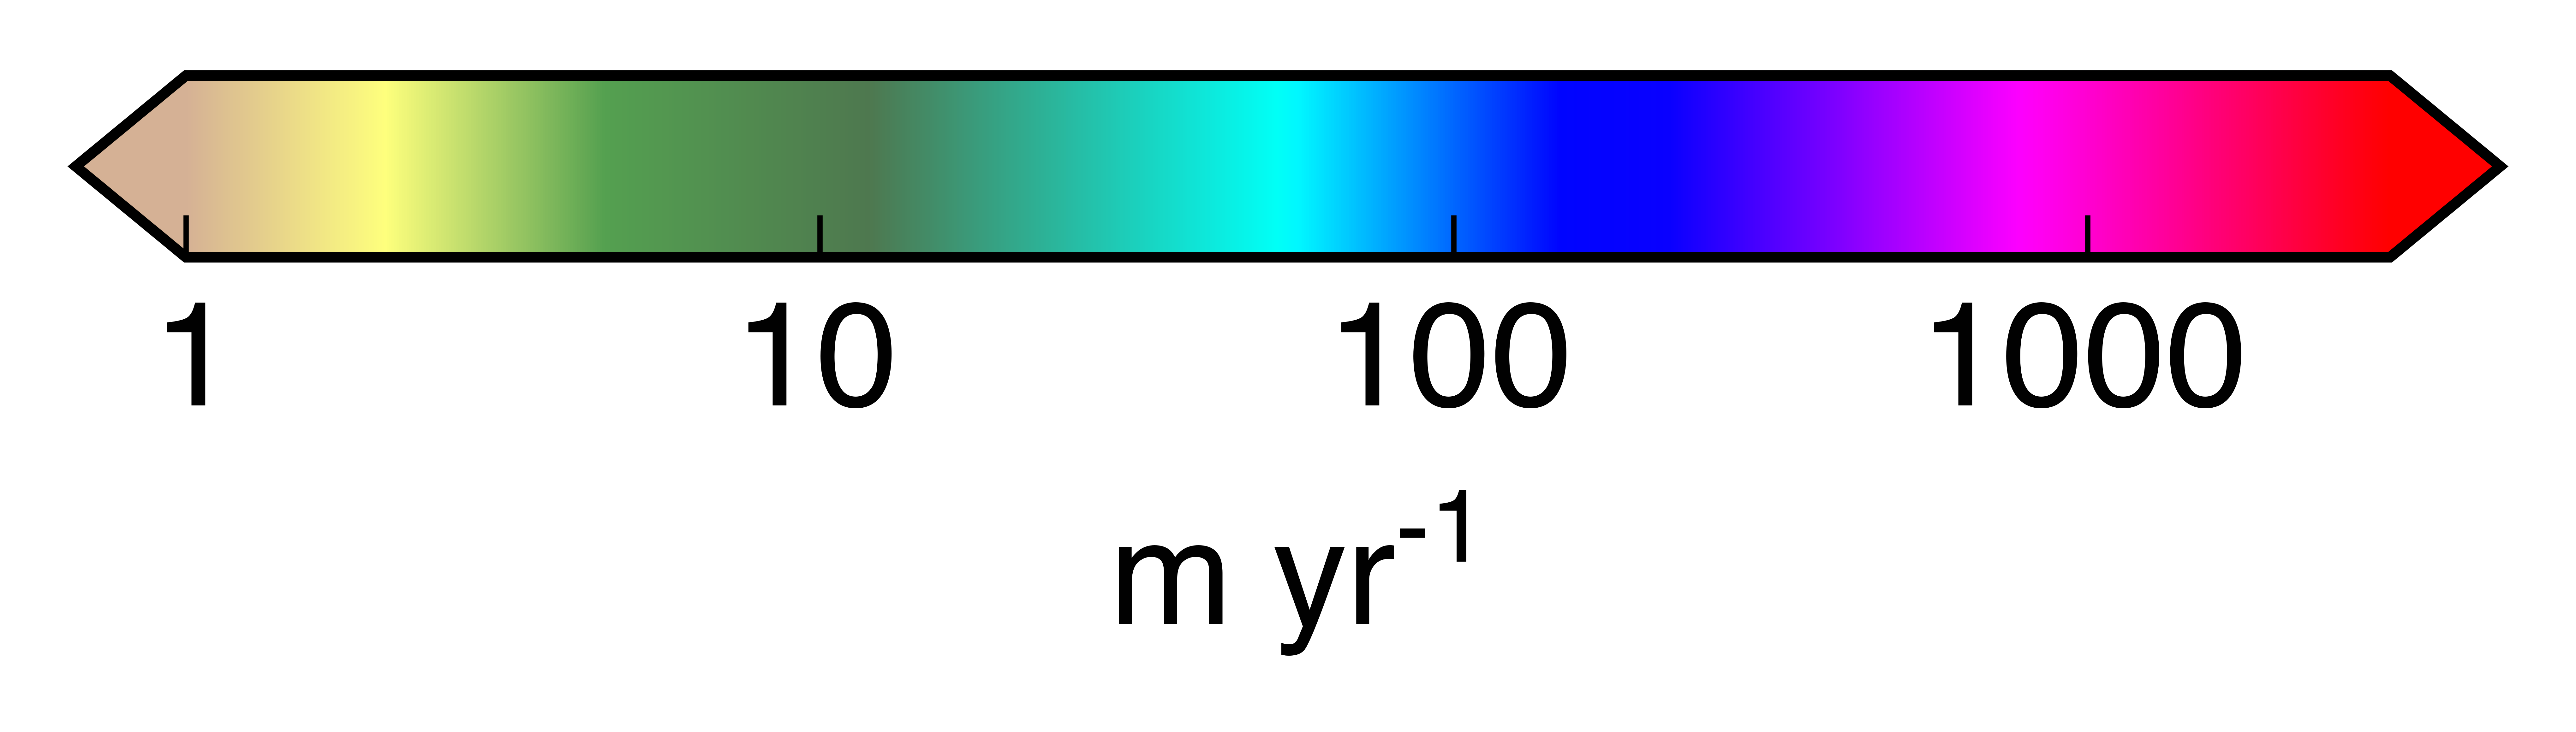
\includegraphics[width=4cm]{colorbar-speed}
  \end{figure}
  \begin{columns}
    \column[T]{5cm}
    \vspace{-2em}
    \begin{figure}
      {\scriptsize{1,200m}\\}
      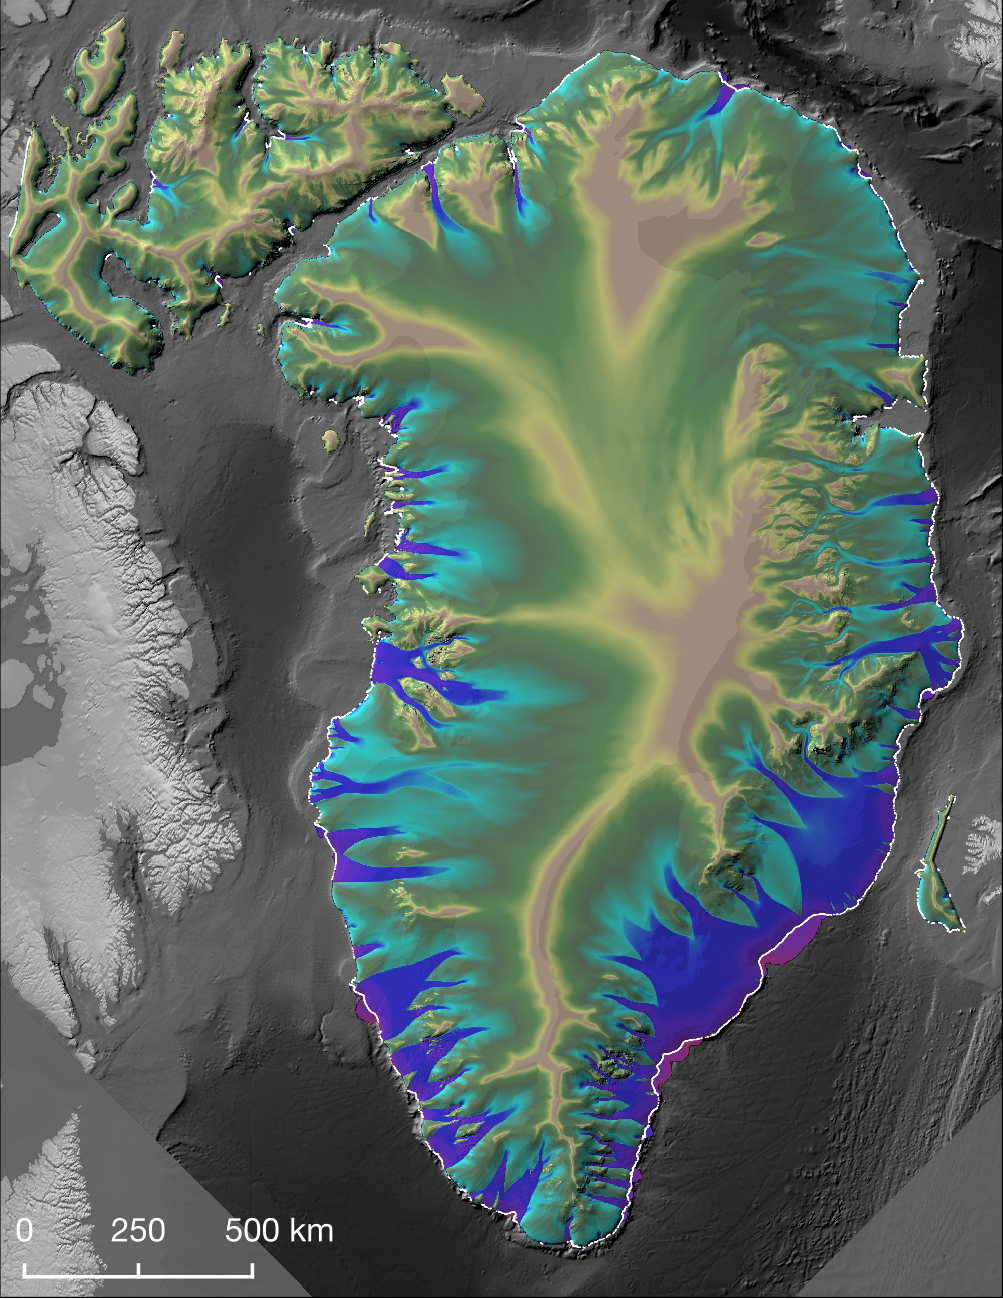
\includegraphics[height=0.7\textheight]{lgm_cc_speed_1200m_ws}
    \end{figure}
    \column[T]{5cm}
    \vspace{-2em}
    \begin{figure}
      {\scriptsize{18,000m, SIA}\\}
      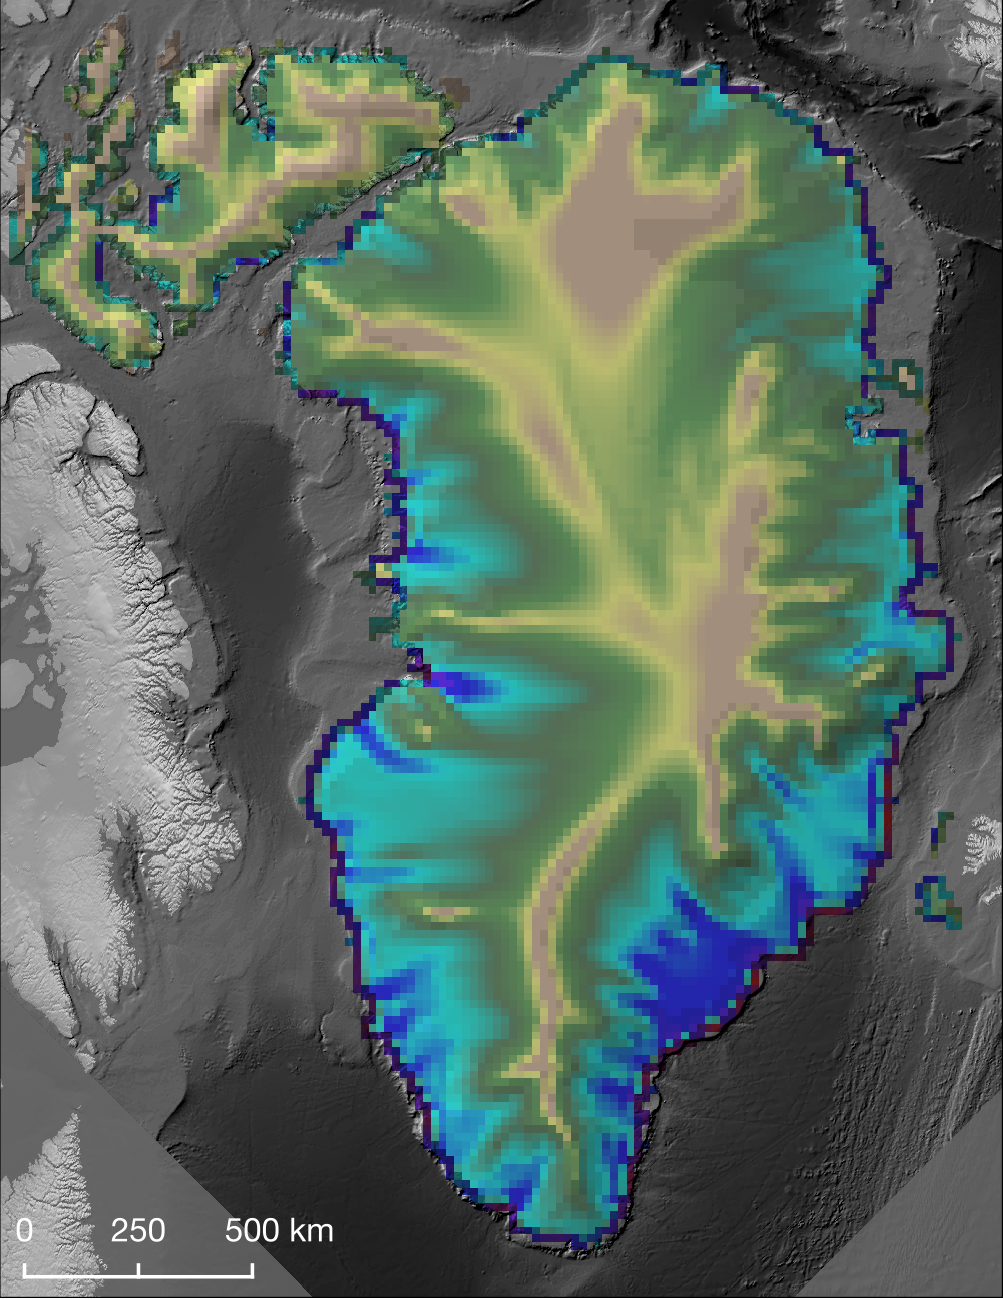
\includegraphics[height=0.7\textheight]{lgm_cc_speed_18000m_sia_ws}
    \end{figure}
  \end{columns}
\end{frame}


\begin{frame}{Funding}
  \begin{figure}
    
\includegraphics[height=2.5cm]{nasa-logo} \hspace{1cm}
    
\includegraphics[height=2.5cm]{NSF-logo-color}
  \end{figure}
\begin{itemize}
\item 2017--2019: project-specific (i.e. non-ISMIP6) support from NASA and NSF
\item until May 2017: full NASA MAP support for Programmer Khroulev
\item after May 2017: ?? support for Programmer Khroulev
\end{itemize}
\end{frame}


\end{document}

